\documentclass[../practica_02.tex]{subfiles}

\begin{document}

    \begin{enumerate}
        \item 
            \begin{itemize}
                \item $x = 3-4t \Rightarrow \star: \frac{-x+3}{4} = t$
                \item $y = 2-3t \stackrel{\star}{\Rightarrow} $
                        $ y = 2 - 3(\frac{-x+3}{4}) \equiv $
                        $ y = \frac{3x}{4} - \frac{1}{4} $
            \end{itemize}

            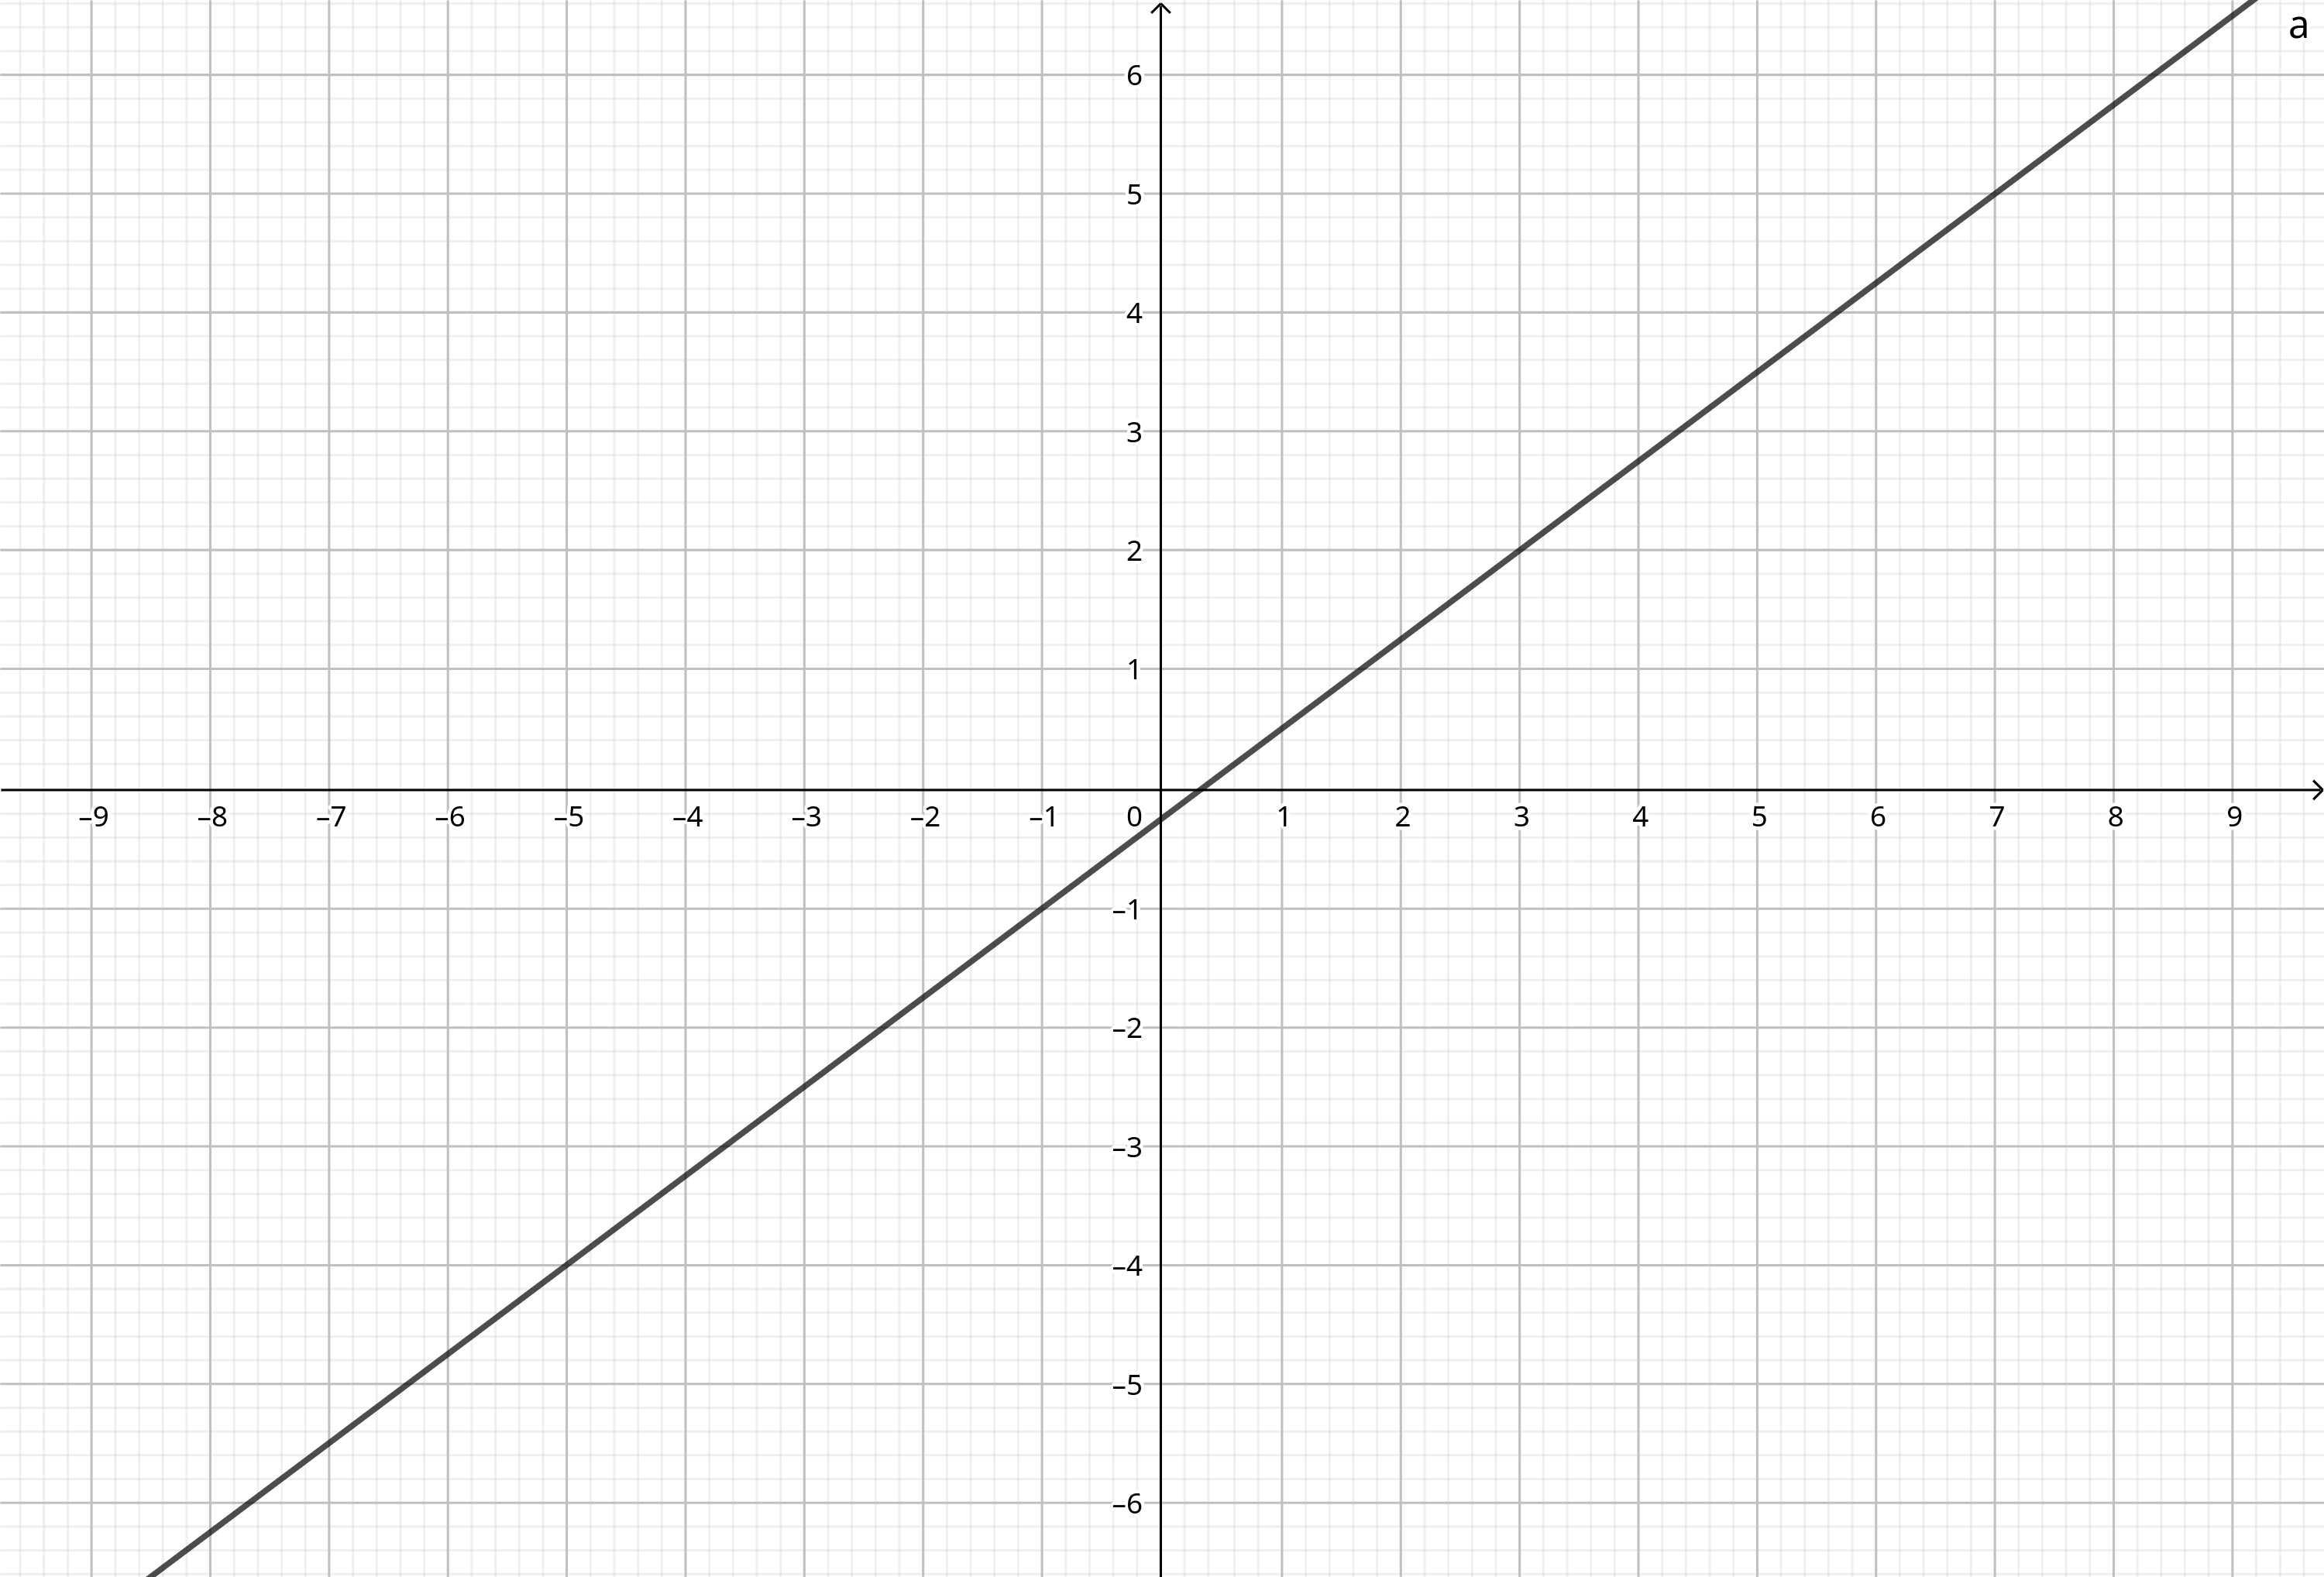
\includegraphics[scale=0.2]{ej01/resources/ej01a.png} $ $
        \item 
            \begin{itemize}
                \item $x = 1-t^2$
                \item $y = t-2$
                \item $-2 \leq t \leq 2$
                \item No es función
            \end{itemize}

            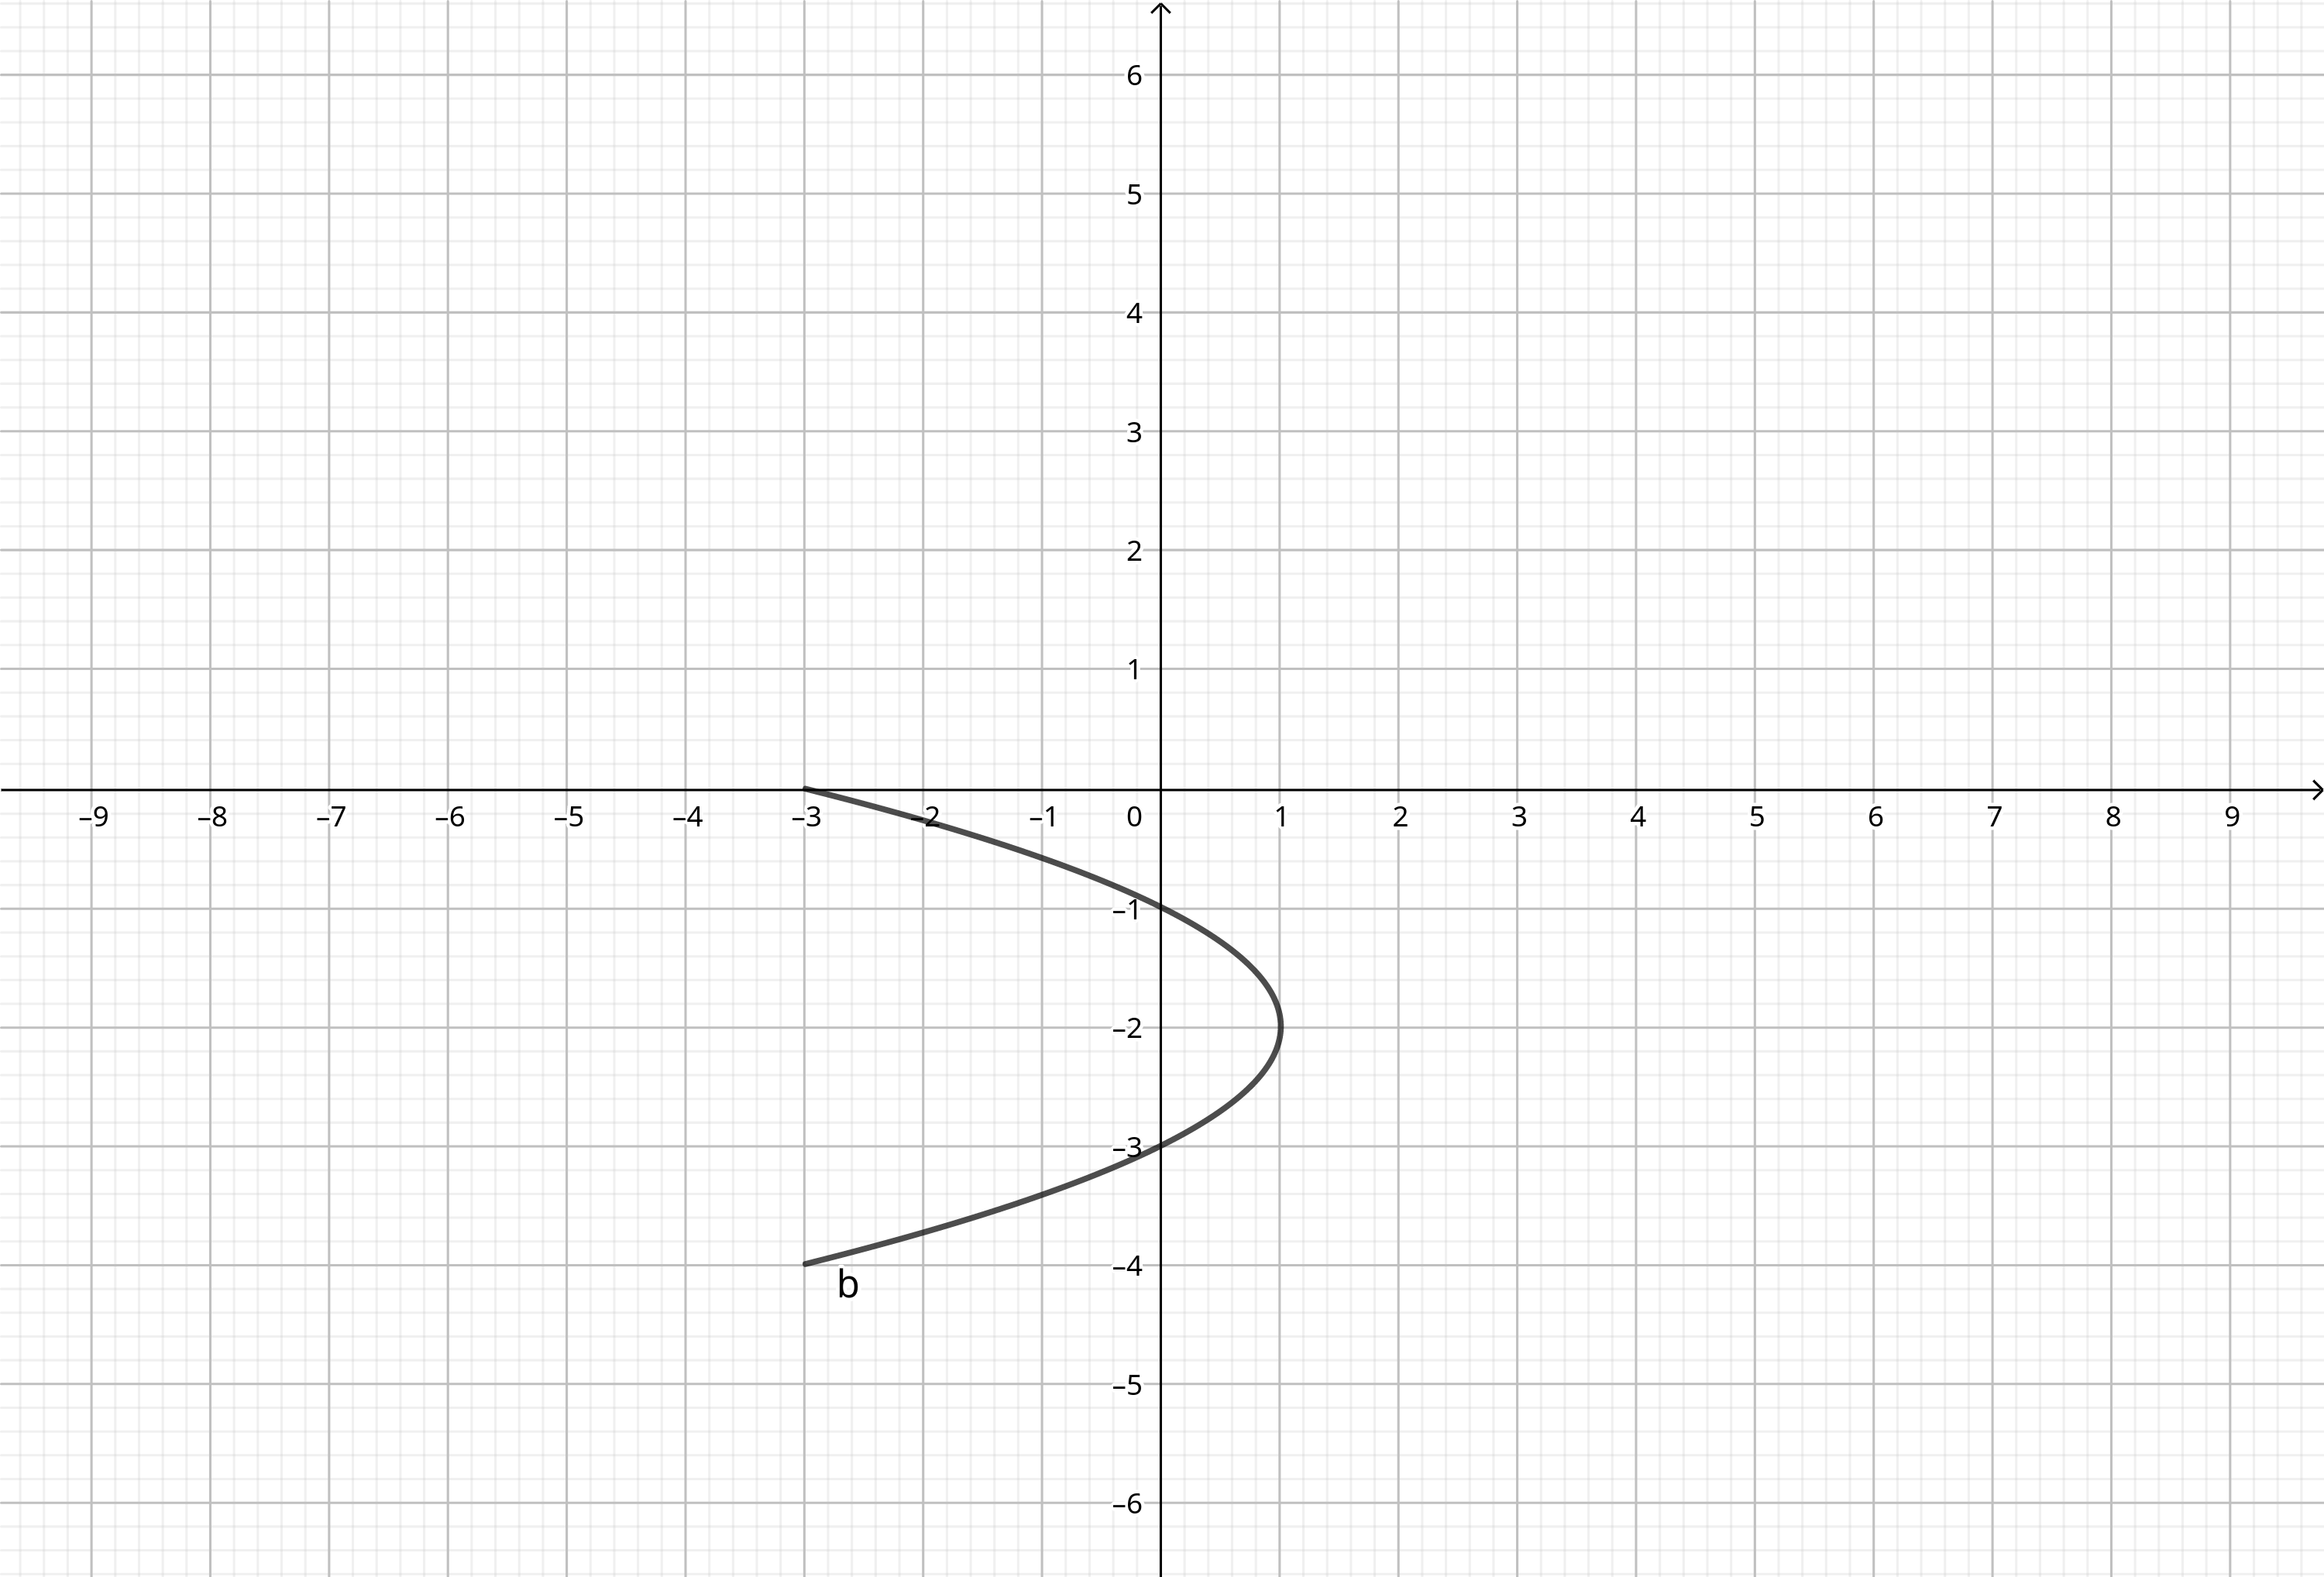
\includegraphics[scale=0.2]{ej01/resources/ej01b.png} $ $
        \item 
            \begin{itemize}
                \item $x = t^2+t$
                \item $y = t^2-t$
                \item $-2 \leq t \leq 2$
                \item No es función
            \end{itemize}

            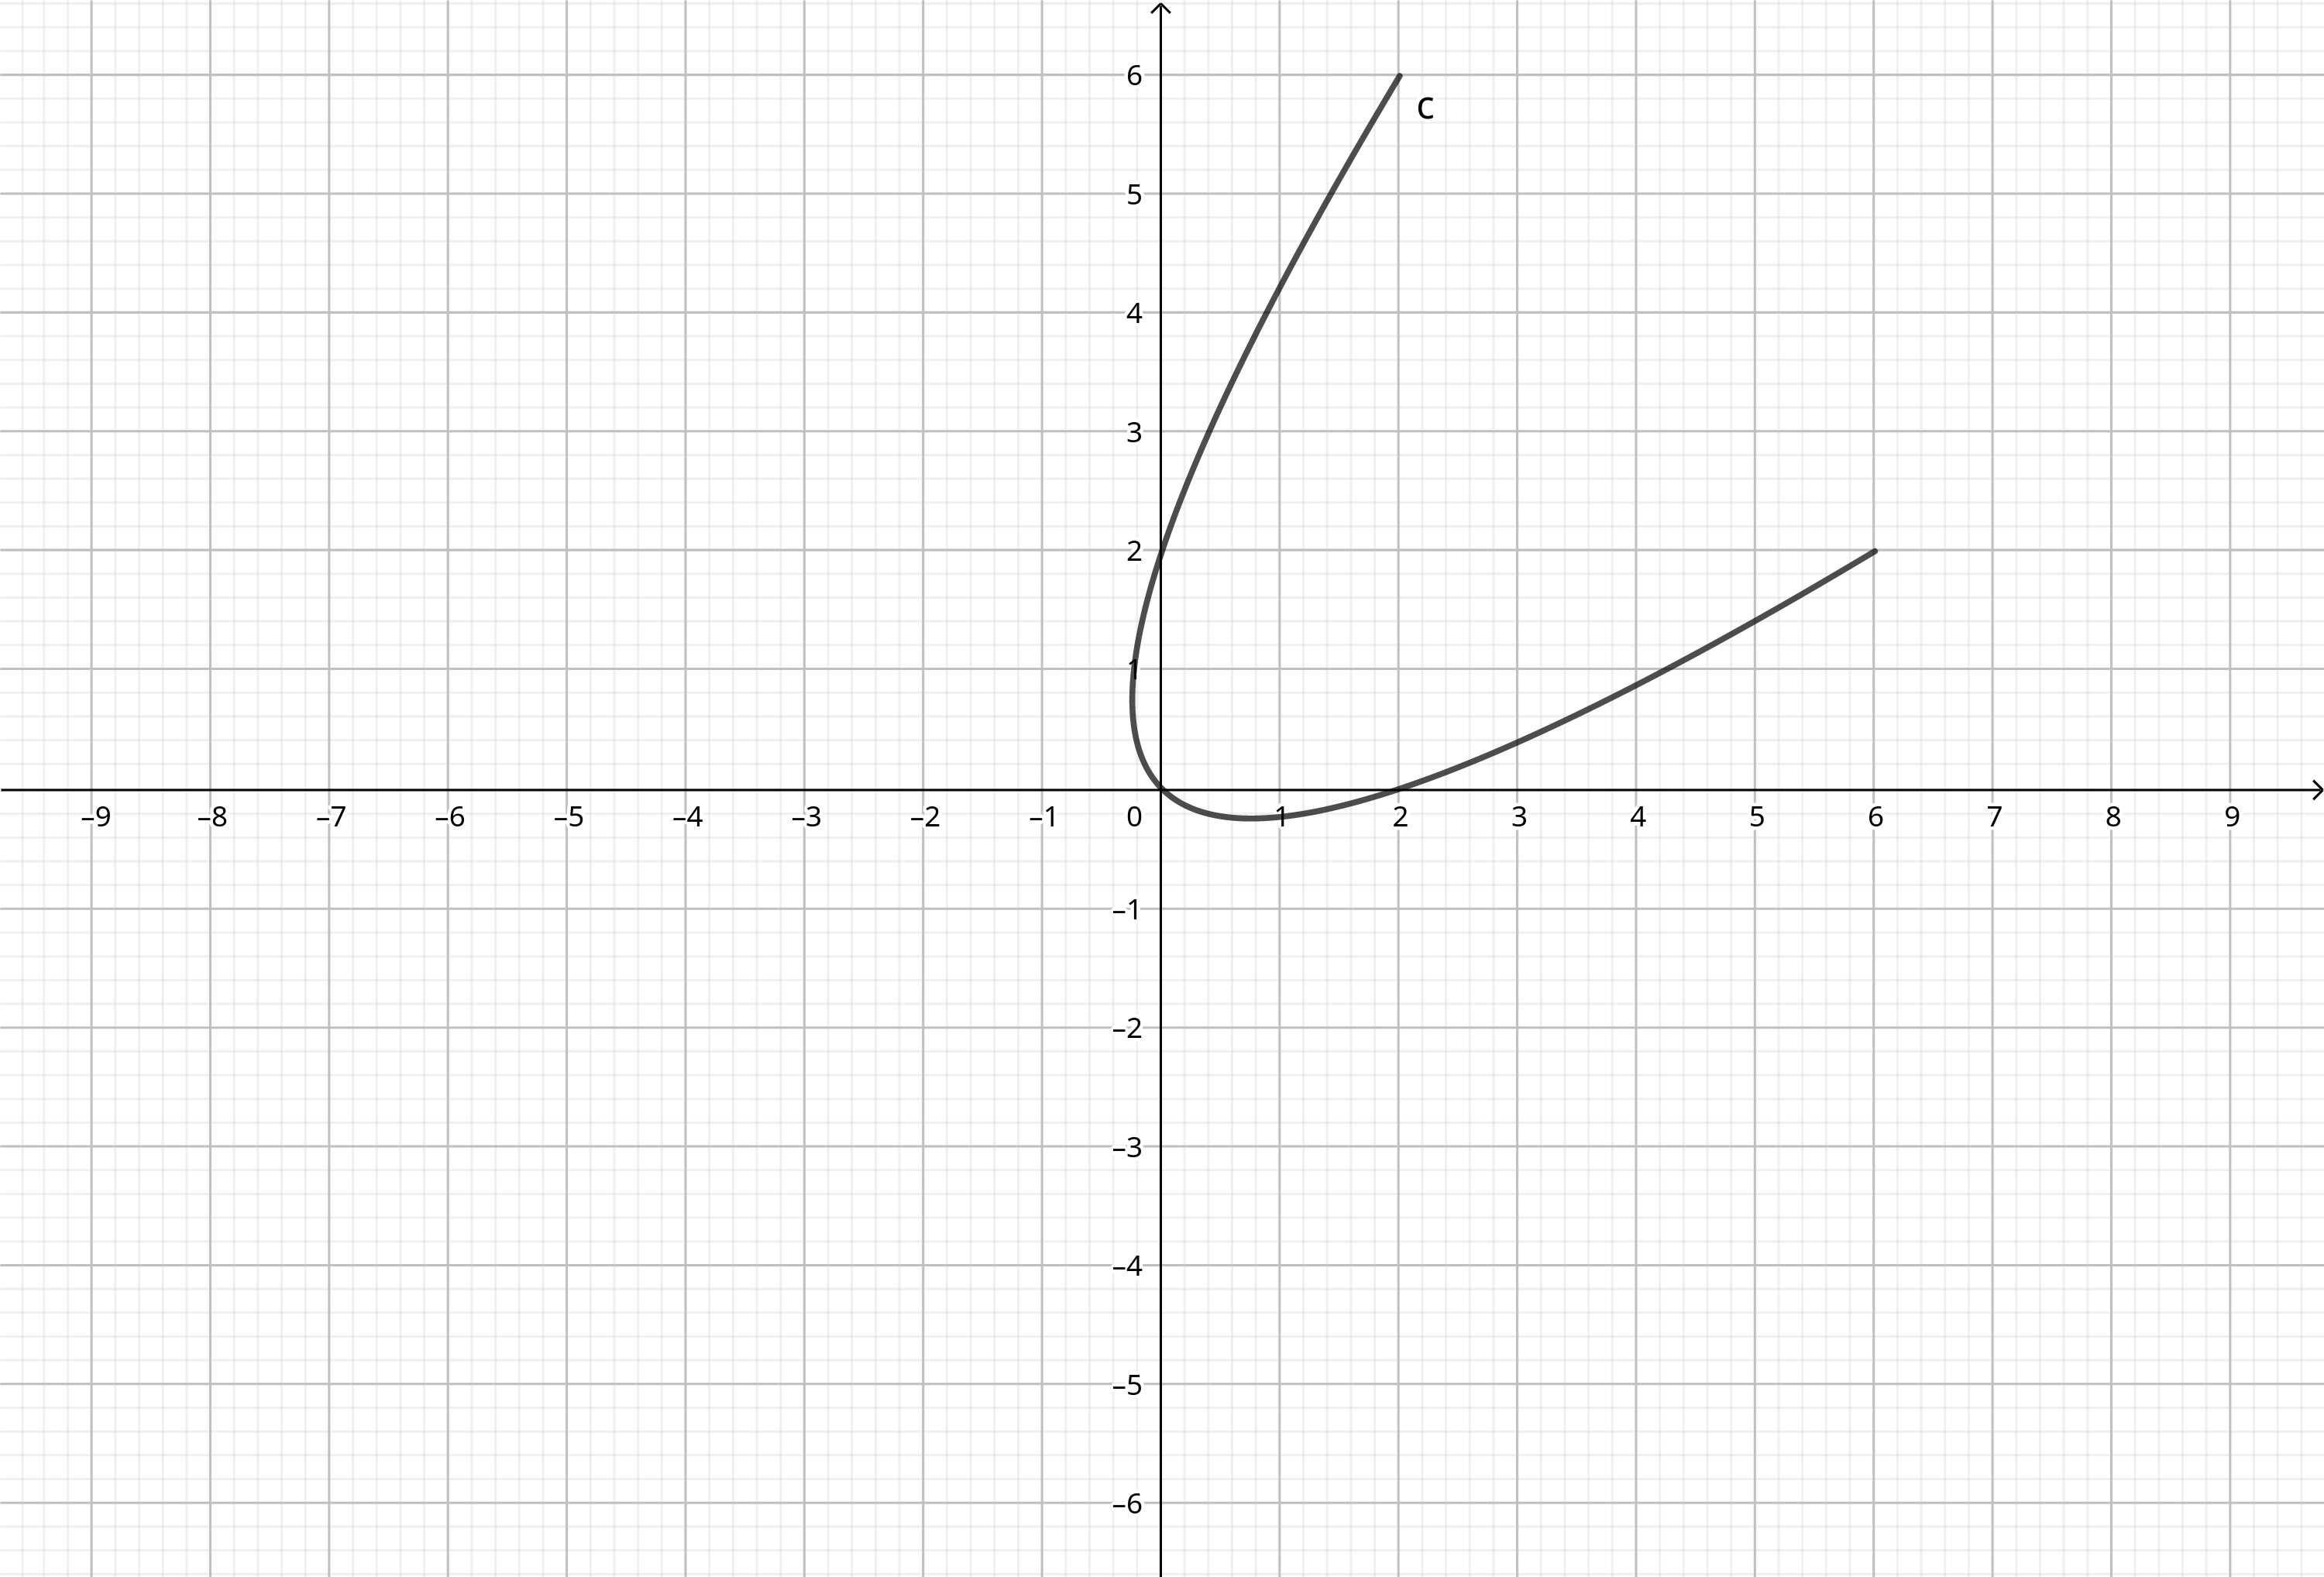
\includegraphics[scale=0.2]{ej01/resources/ej01c.png} $ $
        \item 
            \begin{itemize}
                \item $x = t^2$
                \item $y = t^3-4t$
                \item $-3 \leq t \leq 3$
                \item No es función
            \end{itemize}

            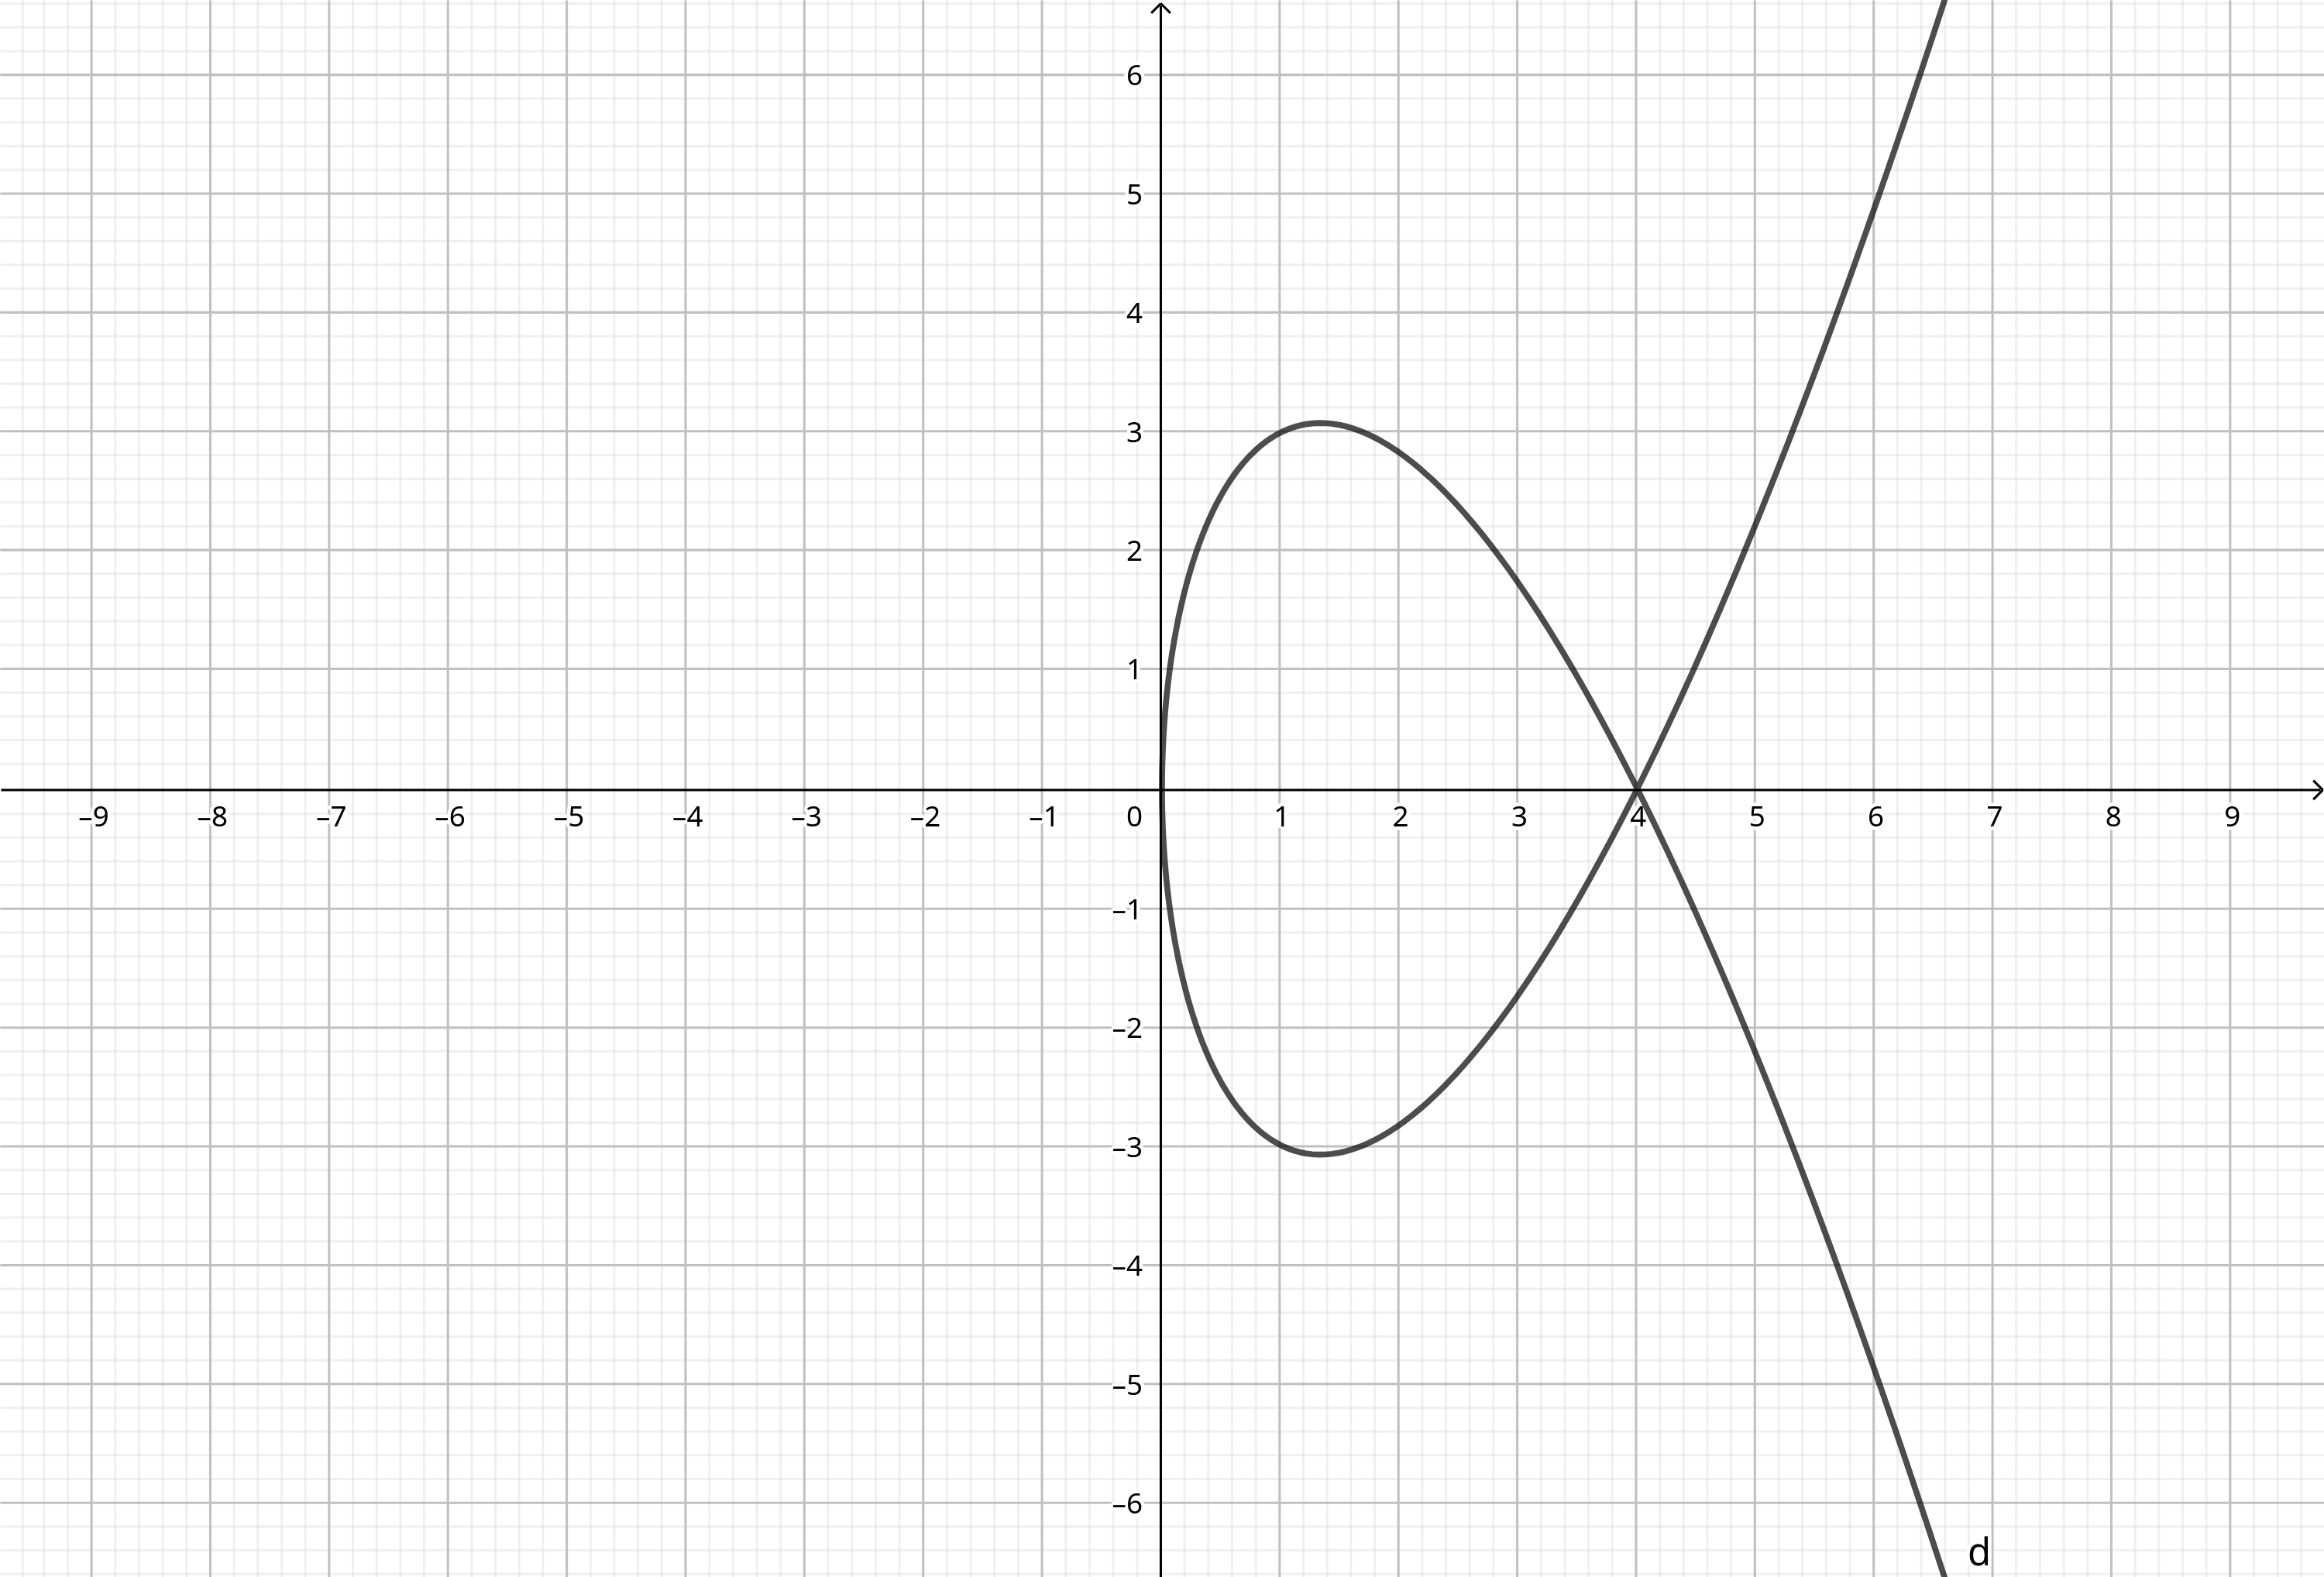
\includegraphics[scale=0.2]{ej01/resources/ej01d.png} $ $
    \end{enumerate}


\end{document}